\documentclass[
  bibliography=totoc,     % Literatur im Inhaltsverzeichnis
  captions=tableheading,  % Tabellenüberschriften
  titlepage=firstiscover, % Titelseite ist Deckblatt
]{scrartcl}

% Paket float verbessern
\usepackage{scrhack}

% Warnung, falls nochmal kompiliert werden muss
\usepackage[aux]{rerunfilecheck}

% unverzichtbare Mathe-Befehle
\usepackage{amsmath}
% viele Mathe-Symbole
\usepackage{amssymb}
% Erweiterungen für amsmath
\usepackage{mathtools}

% Fonteinstellungen
\usepackage{fontspec}
% Latin Modern Fonts werden automatisch geladen
% Alternativ zum Beispiel:
%\setromanfont{Libertinus Serif}
%\setsansfont{Libertinus Sans}
%\setmonofont{Libertinus Mono}

% Wenn man andere Schriftarten gesetzt hat,
% sollte man das Seiten-Layout neu berechnen lassen
\recalctypearea{}

% deutsche Spracheinstellungen
\usepackage[ngerman]{babel}


\usepackage[
  math-style=ISO,    % ┐
  bold-style=ISO,    % │
  sans-style=italic, % │ ISO-Standard folgen
  nabla=upright,     % │
  partial=upright,   % ┘
  warnings-off={           % ┐
    mathtools-colon,       % │ unnötige Warnungen ausschalten
    mathtools-overbracket, % │
  },                       % ┘
]{unicode-math}

% traditionelle Fonts für Mathematik
\setmathfont{Latin Modern Math}
% Alternativ zum Beispiel:
%\setmathfont{Libertinus Math}

\setmathfont{XITS Math}[range={scr, bfscr}]
\setmathfont{XITS Math}[range={cal, bfcal}, StylisticSet=1]

% Zahlen und Einheiten
\usepackage[
  locale=DE,                   % deutsche Einstellungen
  separate-uncertainty=true,   % immer Unsicherheit mit \pm
  per-mode=symbol-or-fraction, % / in inline math, fraction in display math
]{siunitx}

% chemische Formeln
\usepackage[
  version=4,
  math-greek=default, % ┐ mit unicode-math zusammenarbeiten
  text-greek=default, % ┘
]{mhchem}

% richtige Anführungszeichen
\usepackage[autostyle]{csquotes}

% schöne Brüche im Text
\usepackage{xfrac}

% Standardplatzierung für Floats einstellen
\usepackage{float}
\floatplacement{figure}{htbp}
\floatplacement{table}{htbp}

% Floats innerhalb einer Section halten
\usepackage[
  section, % Floats innerhalb der Section halten
  below,   % unterhalb der Section aber auf der selben Seite ist ok
]{placeins}

% Seite drehen für breite Tabellen: landscape Umgebung
\usepackage{pdflscape}

% Captions schöner machen.
\usepackage[
  labelfont=bf,        % Tabelle x: Abbildung y: ist jetzt fett
  font=small,          % Schrift etwas kleiner als Dokument
  width=0.9\textwidth, % maximale Breite einer Caption schmaler
]{caption}
% subfigure, subtable, subref
\usepackage{subcaption}

% Grafiken können eingebunden werden
\usepackage{graphicx}

% schöne Tabellen
\usepackage{booktabs}

% Verbesserungen am Schriftbild
\usepackage{microtype}

% Literaturverzeichnis
\usepackage[
  backend=biber,
]{biblatex}
% Quellendatenbank
\addbibresource{lit.bib}
\addbibresource{programme.bib}

% Hyperlinks im Dokument
\usepackage[
  german,
  unicode,        % Unicode in PDF-Attributen erlauben
  pdfusetitle,    % Titel, Autoren und Datum als PDF-Attribute
  pdfcreator={},  % ┐ PDF-Attribute säubern
  pdfproducer={}, % ┘
]{hyperref}
% erweiterte Bookmarks im PDF
\usepackage{bookmark}

% Trennung von Wörtern mit Strichen
\usepackage[shortcuts]{extdash}

\author{%
  Felix Symma\\%
  \href{mailto:felix.symma@tu-dortmund.de}{felix.symma@tu-dortmund.de}%
  \and%
  Joel Koch\\%
  \href{mailto:joel.koch@tu-dortmund.de}{joel.koch@tu-dortmund.de}%
}
\publishers{TU Dortmund – Fakultät Physik}

\subject{V308}
\title{Magnetfelder und Spulen}
\date{%
  Durchführung: 16.11.2021
  \hspace{3em}
  Abgabe: 23.11.2021
}

\begin{document}
\setlength{\parindent}{0pt} %verhindert das Einrücken

\maketitle
\thispagestyle{empty}
\tableofcontents
\newpage
%was noch zu tun ist: 
%Diskussion schreiben (Abweichungen von der Theorie zeigen, die man auf den Diagrammen sehen kann)
%Literaturverzeichnis->erledigt
%Theoriewert für lange Spule bei auswertung hinzufügen-->nicht möglich, weil Messwert fehlt
%evtl. Eckdaten der einzelnen Spulen noch hinzufügen (Windungszahl, Durchmesser, ...)-->erledigt
%hab zwei graphiken noch in eine subfigure gepackt, damit nicht der ganze platz davon eingenommen wird
%hab dir teilweise geantwortet in theorie.tex (kommentare mit @R: damit du sie leichter finden kannst ;) )

\section{Einleitung}
\label{sec:Einleitung}
Ziel des Versuches ist es gekoppelte Schwingkreise zu untersuchen. Obwohl im folgenden ein elektromaknetischer
Schwingkreis betrachtet wird, lassen sich die Erkenntnisse leicht auf ein mechanisches Analogon übertragen
(zum Beispiel ein gekoppeltes Schwingungssystem, bestehend aus 2 Fadenpendeln, die über eine elastische Feder miteinander verbunden sind 
\cite{Versuchsanleitung}). Der Grund, dass am elektrischen Schwingkreis Untersuchungen vorgenommen werden, ist dass die Amplitude und die Frequenz
einfacher und genauer bestimmt werden können.
Bei der Beobachtung des Schwingkreises wird auf die Energieverteilung der Systeme und auf den Einfluss
eines äußeren Erregers auf das schwingende System geachtet.

Die Erkenntnisse werden anschließend ausgewertet und mit der Theorie abgeglichen.
\section{Theorie}
\label{sec:Theorie}

Ein Trägheitsmoment ist immer bezüglich einer Achse definiert, um die sich das zu beobachtende Objekt dreht.
Dreht sich ein ausgedehnter Körper um eine feste Achse, so dreht sich jedes einzelne Massenelement $m_i$ des Körpers
und es folgt das Gesamtträgheitsmoment des Körpers zu

\begin{equation*}
    \label{eqn:traegheitsm}
    I = \sum_i r_i^2 \cdot m_i.
\end{equation*}

\noindent
Dabei ist $r_i$ der Abstand des i-ten Massenelements $m_i$ senkrecht zur Drehachse.
Für unendlich viele infinitesimal kleine Massenelemente geht die Gleichung \autoref{eqn:traegheitsm} in die Relation 

\begin{equation*}
    \label{eqn:traegheitsmoment}
    I = \int r_{\perp}^2 \, dm
\end{equation*}

\noindent
über.
Für die Beschreibung komplexerer Körper, wird der beschriebene Körper in einzelne Teilkörper aufgeteilt. Das Gesamtträgheitsmoment ergibt
sich dann als die Summe der Trägheitsmomente der Teilkörper. Dabei ist darauf zu achten, dass alle aufsummierten Körper sich auf die 
gleiche Achse beziehen.
Ist die Drehachse nicht gleich der Schwerpunktsache des Körpers, so liefert der \textit{Steiner'sche Satz} einen Weg zur Berechnung des
Trägheitsmomentes $I$

\begin{equation}
    \label{eqn:steiner}
    I = I_{\text{S}} \, + m a^2,
\end{equation}

\noindent
sofern die beiden Achsen parallel zueinander sind.
Dabei ist $I_{\text{S}}$ das Trägheitsmoment des Körpers bei Drehung um die Schwerpunktsache, $m$ die Masse des Körpers und $a$ der 
Abstand der Schwerpunktsache zur Drehachse. 
\noindent
Wirkt auf einen Körper im Abstand $\vec r$ eine Kraft $\vec F$, so wirkt auf ihn ein \textit{Drehmoment}, was wie folgt defieniert ist.

\begin{equation*}
    \label{eqn:drehmoment}
    \vec M = \vec F\times\vec r
\end{equation*}

\noindent
Eine Spiralfeder, wie sie auch an der Apparatur in dem Versuch angebracht ist, verrichtet ein Drehmoment, das der Auslenkung entgegengerichtet ist.
Es folgt damit der Zusammenhang.
\begin{equation}
    \label{eqn:winkelrichtgr}
    \vec M = -D \vec\varphi    
\end{equation} 
Dabei ist $D$ die Winkelrichtgröße, beziehungsweise der Proportionalitätsfaktor
und $\vec\varphi$ der Auslenkwinkel \cite{gerthsen}.
Unter einer solchen Voraussetzung führt der Körper eine harmonische Schwingung aus, dessen Periodendauer wie folgt lautet.

\begin{equation}
    \label{eqn:periode}
    T=2\pi\sqrt\frac{I}{D}.
\end{equation}

\section{Durchführung}
\label{sec:Durchführung}
Für die Messung der Suszeptibilität wird der in \autoref{fig:blockschaltbild} dargestellte Aufbau verwendet.

\begin{figure}[H]
	\centering
	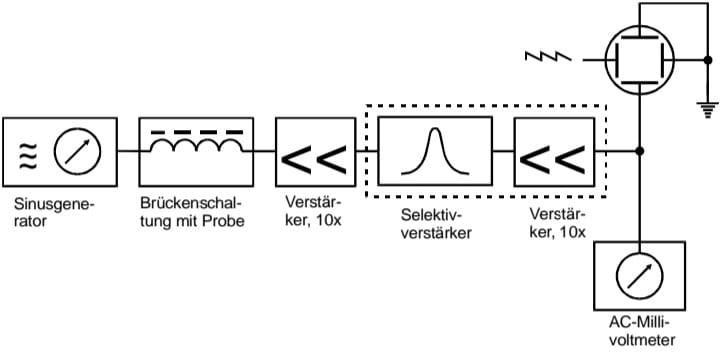
\includegraphics[width=0.6\linewidth]{data/blockschaltbild.jpeg}
	\caption{Blockschaltbild der verwendeten Messapparatur.}
	\label{fig:blockschaltbild}
\end{figure}
\noindent
Da zur Messung eine Brückenschaltung verwendet wird, ensteht an den Ausgängen eine Störspannung, die die eigentliche Brückenspannung komplett überdeckt. Um die Brückenspannung
trotzdem messbar zu machen wird ein Selektivverstärker verwendet, der nur für monofrequente Signalspannungen durchlässsig ist und somit die Brückenspannung herausfiltert. Es wird 
außerdem ein Linearverstärker verwendet, um die kleinen Spannungsänderungen messbar zu machen.
\newline \newline
Im ersten Schritt der Messung wird die Filterkurve des Selektivfilters bestimmt. Hierzu wird die Spannungsquelle direkt mit dem Selektivverstärker verbuden. Es kann nun die Spannungsfrequenz
variiert und die daraus resultierende Ausgangsspannung $U_{\text{A}}$ mit Hilfe eines Millivoltmeters gemessen und notiert werden. Die Messungen wurden in einen Frequenzbereich von 20 bis
$\SI{40}{\kilo\hertz}$ durchgeführt, wobei die Abstände der Messwerte nahe des Peaks der Ausgangsspannung $U_{\text{A}}$ enger gewählt wurden als am Rand des Frequenzbereichs.
\newline \newline
Im zweiten Schritt des Versuches wird nun die eigentliche Suszeptibilitätsmessung durchgeführt. Hierfür wird zunächst die Signalfrequenz auf die Durchlassfrequenz des Selektivverstärkers
eingestellt. Zur Messung werden zwei verschiedene Methoden angewandt. Zum einen wird die Änderung der Brückenspannung gemessen, die auftritt, wenn bei abgeglichener Brücke mit leeren Spulen
die Probe in diese eingeführt wird. Zum anderen wird die Brücke nach Einführung der Probe erneut abgeglichen und die veränderten Werte der Widerstände notiert.
\newline
Beide Verfahren werden jeweils parallel für die drei zu messenden Seltenen Erd-Oxiden $Gd_2O_3$, $Nd_2O_3$ und $Dy_2O_3$ angewandt. Es wird jede Messung drei mal durchgeführt und aus den
Ergebnissen jeweils der Durchschnitt gebildet. Anschließend werden die Längen und Durchmesser der Proben vermesssen.
\section{Auswertung}
\label{sec:Auswertung}

\DeclareSIUnit{\rad}{rad} %Damit "rad" in \SI verwendet werden kann

\subsection{Messung der Zeitkonstanten $RC$ über die Entladekurve}
Die in Aufgabenteil a) verwendete Frequenz beträgt $\SI{420}{\hertz}$. Aus dem Zusammenhang für den Entladevorgang eines Kondenators folgt
\begin{align}
    \symup{ln}(\frac{U}{U_{0}}) = -\frac{1}{RC}\cdot t.
\end{align}
Mithilfe von numpy \cite{numpy} und matplotlib \cite{matplotlib} werden die Messwerte, die
\autoref{tab:wertea} zu entnehmen sind, halblogarithmisch in \autoref{fig:plot_a} geplottet und es wird eine Regressionsgerade erstellt.

\begin{table}[H]
    \centering
    \caption{Messwerte zu Aufgabe a).}
    \label{tab:wertea}
    \begin{tabular}{c c}
        \toprule
        $U \:/\:$ V & $t \:/\:$ ms \\
        \midrule
        0,55 & 0,00 \\
        0,50 & 0,02 \\
        0,44 & 0,04 \\
        0,40 & 0,05 \\
        0,36 & 0,06 \\
        0,32 & 0,08 \\
        0,26 & 0,10 \\
        0,24 & 0,12 \\
        0,18 & 0,14 \\
        0,12 & 0,16 \\
        0,1 & 0,18 \\
        0,04 & 0,20 \\
        0,00 & 0,22 \\
        -0,04 & 0,24 \\
        -0,06 & 0,26 \\
        -0,10 & 0,28 \\
        -0,14 & 0,30 \\
        -0,16 & 0,32 \\
        -0,18 & 0,34 \\
        -0,22 & 0,36 \\
        -0,24 & 0,38 \\
        -0,28 & 0,40 \\
        -0,30 & 0,42 \\
        -0,32 & 0,44 \\
        -0,34 & 0,46 \\
        -0,38 & 0,48 \\
        -0,40 & 0,5 \\
        -0,42 & 0,52 \\
        -0,44 & 0,54 \\
        -0,46 & 0,56 \\
        -0,48 & 0,58 \\
        -0,50 & 0,6 \\
        \bottomrule
    \end{tabular}
\end{table}

\begin{figure}[H]
    \centering
    \includegraphics{build/plota.pdf}
    \caption{Halblogarithmischer Plot zu Aufgabenteil a) mit Ausgleichsgerade.}
    \label{fig:plot_a}
  \end{figure}

Die Parameter der Ausgleichsgeraden vom Typ $\symup{ln}(\frac{U}{U_{0}}) = m \cdot t + b$ werden zu den folgenden Werten ermittelt
\begin{align*}
    m = \SI{-0.697 (0.014)}{\per\milli\second}, \\
    b = 1.087 \.\pm 0.014. \\
\end{align*}
Dadrch ergibt sich eine Zeitkonstante $RC$ von 
\begin{align*}
    RC = \SI{0.705 (0.014)}{\per\second}.
\end{align*}



\subsection{Bestimmen der Zeitkonstanten $RC$ über die Frequenzabhängigkeit der Amplitude}
Aus \autoref{tab:wertebc} sind die Messwerte zu Aufgabenteil b) und c) zu entnehmen.
\begin{table}[H]
    \centering
    \caption{Messwerte zu Aufgabe b) und c).}
    \label{tab:wertebc}
    \begin{tabular}{c c c c c}
        \toprule
        $f \:/\:\si{\kilo\hertz}$ & $A_1 \:/\: \si{\volt}$ & $A_1 \:/\: \si{\volt}$ & $a \:/\: \si{\milli\second}$ & $b \:/\: \si{\milli\second}$ \\
        \midrule
        3,085 & 4,2 & 0,1100 & 0,0300 & 0,1800 \\
        6 & 4,2 & 0,0600 & 0,0240 & 0,0680 \\
        9 & 4,2 & 0,0480 & 0,0180 & 0,070 \\
        12 & 4,2 & 0,0360 & 0,0120 & 0,0460 \\
        15 & 4,2 & 0,0260 & 0,0100 & 0,0380 \\
        18 & 4,2 & 0,0220 & 0,0100 & 0,0240 \\
        21 & 4,2 & 0,0180 & 0,0080 & 0,0260 \\
        24 & 4,2 & 0,0150 & 0,0070 & 0,0230 \\
        27 & 4,2 & 0,0130 & 0,0060 & 0,0210 \\
        30 & 4,2 & 0,0110 & 0,0050 & 0,0190 \\
        33 & 4,2 & 0,0100 & 0,0050 & 0,0165 \\
        36 & 4,2 & 0,0085 & 0,0050 & 0,0150 \\
        39 & 4,2 & 0,0075 & 0,0045 & 0,0114 \\
        42 & 4,2 & 0,0070 & 0,0040 & 0,0135 \\
        45 & 4,2 & 0,0060 & 0,0040 & 0,0120 \\
        48 & 4,2 & 0,0060 & 0,0035 & 0,0115 \\
        51 & 4,2 & 0,0050 & 0,0030 & 0,0110 \\
        54 & 4,2 & 0,0050 & 0,0030 & 0,0100 \\
        57 & 4,2 & 0,0045 & 0,0030 & 0,0100 \\
        60 & 4,2 & 0,0040 & 0,0025 & 0,0095 \\
        \bottomrule
    \end{tabular}
\end{table}


\begin{figure}[H]
    \centering
    \includegraphics[width=0.75\textwidth]{build/plotb.pdf}
    \caption{Frequenzabhängiges Amplitudenverhältnis.}
    \label{fig:Plotb}
\end{figure}
Aus (\ref{eqn:Amplitude}) ergibt sich ein Zusammenhang für die Ausgleichsrechnung der Zeitkonstanten $RC$
\begin{align}
    \frac{A(\omega)}{U_0} = \frac{1}{\sqrt{1+\omega^2R^2C^2}}.
    \label{eqn:ausgl}
\end{align}
Aus \autoref{fig:Plotb} ist die graphische Abbildung der Messwerte aus \autoref{tab:wertebc} zu entnehmen, wodurch mithilfe der Python
Erweiterungen matplotlib \cite{matplotlib}, numpy \cite{numpy} und scipy \cite{scipy} die Zeitkonstanten $RC$ bestimmt wird.
Es folgt eine Zeitkonstante von
\begin{align*}
    RC = \SI{1.88 (1.55)}{\per\second}.
\end{align*}

\subsection{Phasenverschiebung des RC-Kreises}
Ein Zusammenhang zwischen der Phasenverschiebung von $U_{\text{C}}$ und $U_0$ und der Frequenz der Spannungsquelle wird durch
die folgende Gleichung beschrieben
\begin{align}
    \varphi(\omega) = -\arctan{-\omega\cdot RC}.
    \label{eqn:phasev}
\end{align}
Dabei wird die Phase über $\varphi = 2\pi\frac ab$ bestimmt. Die Messwerte sind \autoref{tab:wertebc} zu entnehmen.
Das Wertepaar $\{f\,[\si{\hertz}], \varphi(\omega)\, [\si{\rad}]\}$ wird in \autoref{fig:plotc} dargestellt.
\begin{figure}[H]
    \centering
    \includegraphics[width=0.75\textwidth]{build/plotc.pdf}
    \caption{Graphische Darstellung der Phasenverschiebung.}
    \label{fig:plotc}
\end{figure}
Es ist jedoch nicht möglich aus den gemessenen Werten eine Zeitkonstante $RC$ zu bestimmen, worauf näher in \autoref{sec:Diskussion}
eingegangen wird.

Die Werte werden zusätzlich in einem Polarplot in \autoref{fig:plotd} visualisiert, aus dem sich aus denselben Gründen 
keine Informationen entnehmen lassen.
\begin{figure}[H]
    \centering
    \includegraphics[width=0.75\textwidth]{build/plotd.pdf}
    \caption{Polarplot zu der Phasenverschiebung $\varphi$.}
    \label{fig:plotd}
\end{figure}

\subsection{RC-Kreis als Integrator}
\label{subsec:integr}
Aus \autoref{subsec:int} folgt, dass ein RC-Kreis auch als Integrator dienen kann.
Für eine Rechteckspannung mit konstanten Spannungsabschnitten ist eine Stammfunktion mit einem linearen Spannungsbild zu erwarten.
In \autoref{fig:d.3} ist ebendies dargestellt.
Bei einer angelegten Dreiecksspannung mit linearem Verlauf ist ein quadratischer Spannungsverlauf zu erwarten.
Durch den zeitlichen Verlauf ergibt sich somit eine sinusförmiger Spannungsverlauf, wie er in \autoref{fig:d.2} dargestellt ist.
Durch Integration einer Sinusspannung der Form 
\begin{align*}
    f(\omega) = \sin{\omega t},
\end{align*}
ist eine Cosinunsspannung der Form
\begin{align*}
    f(\omega) = \frac{1}{\omega} \cos{\omega t}
\end{align*}
zu erwarten, was in \autoref{fig:d.1} abgebildet wird.
\begin{figure}[H]
    \centering
    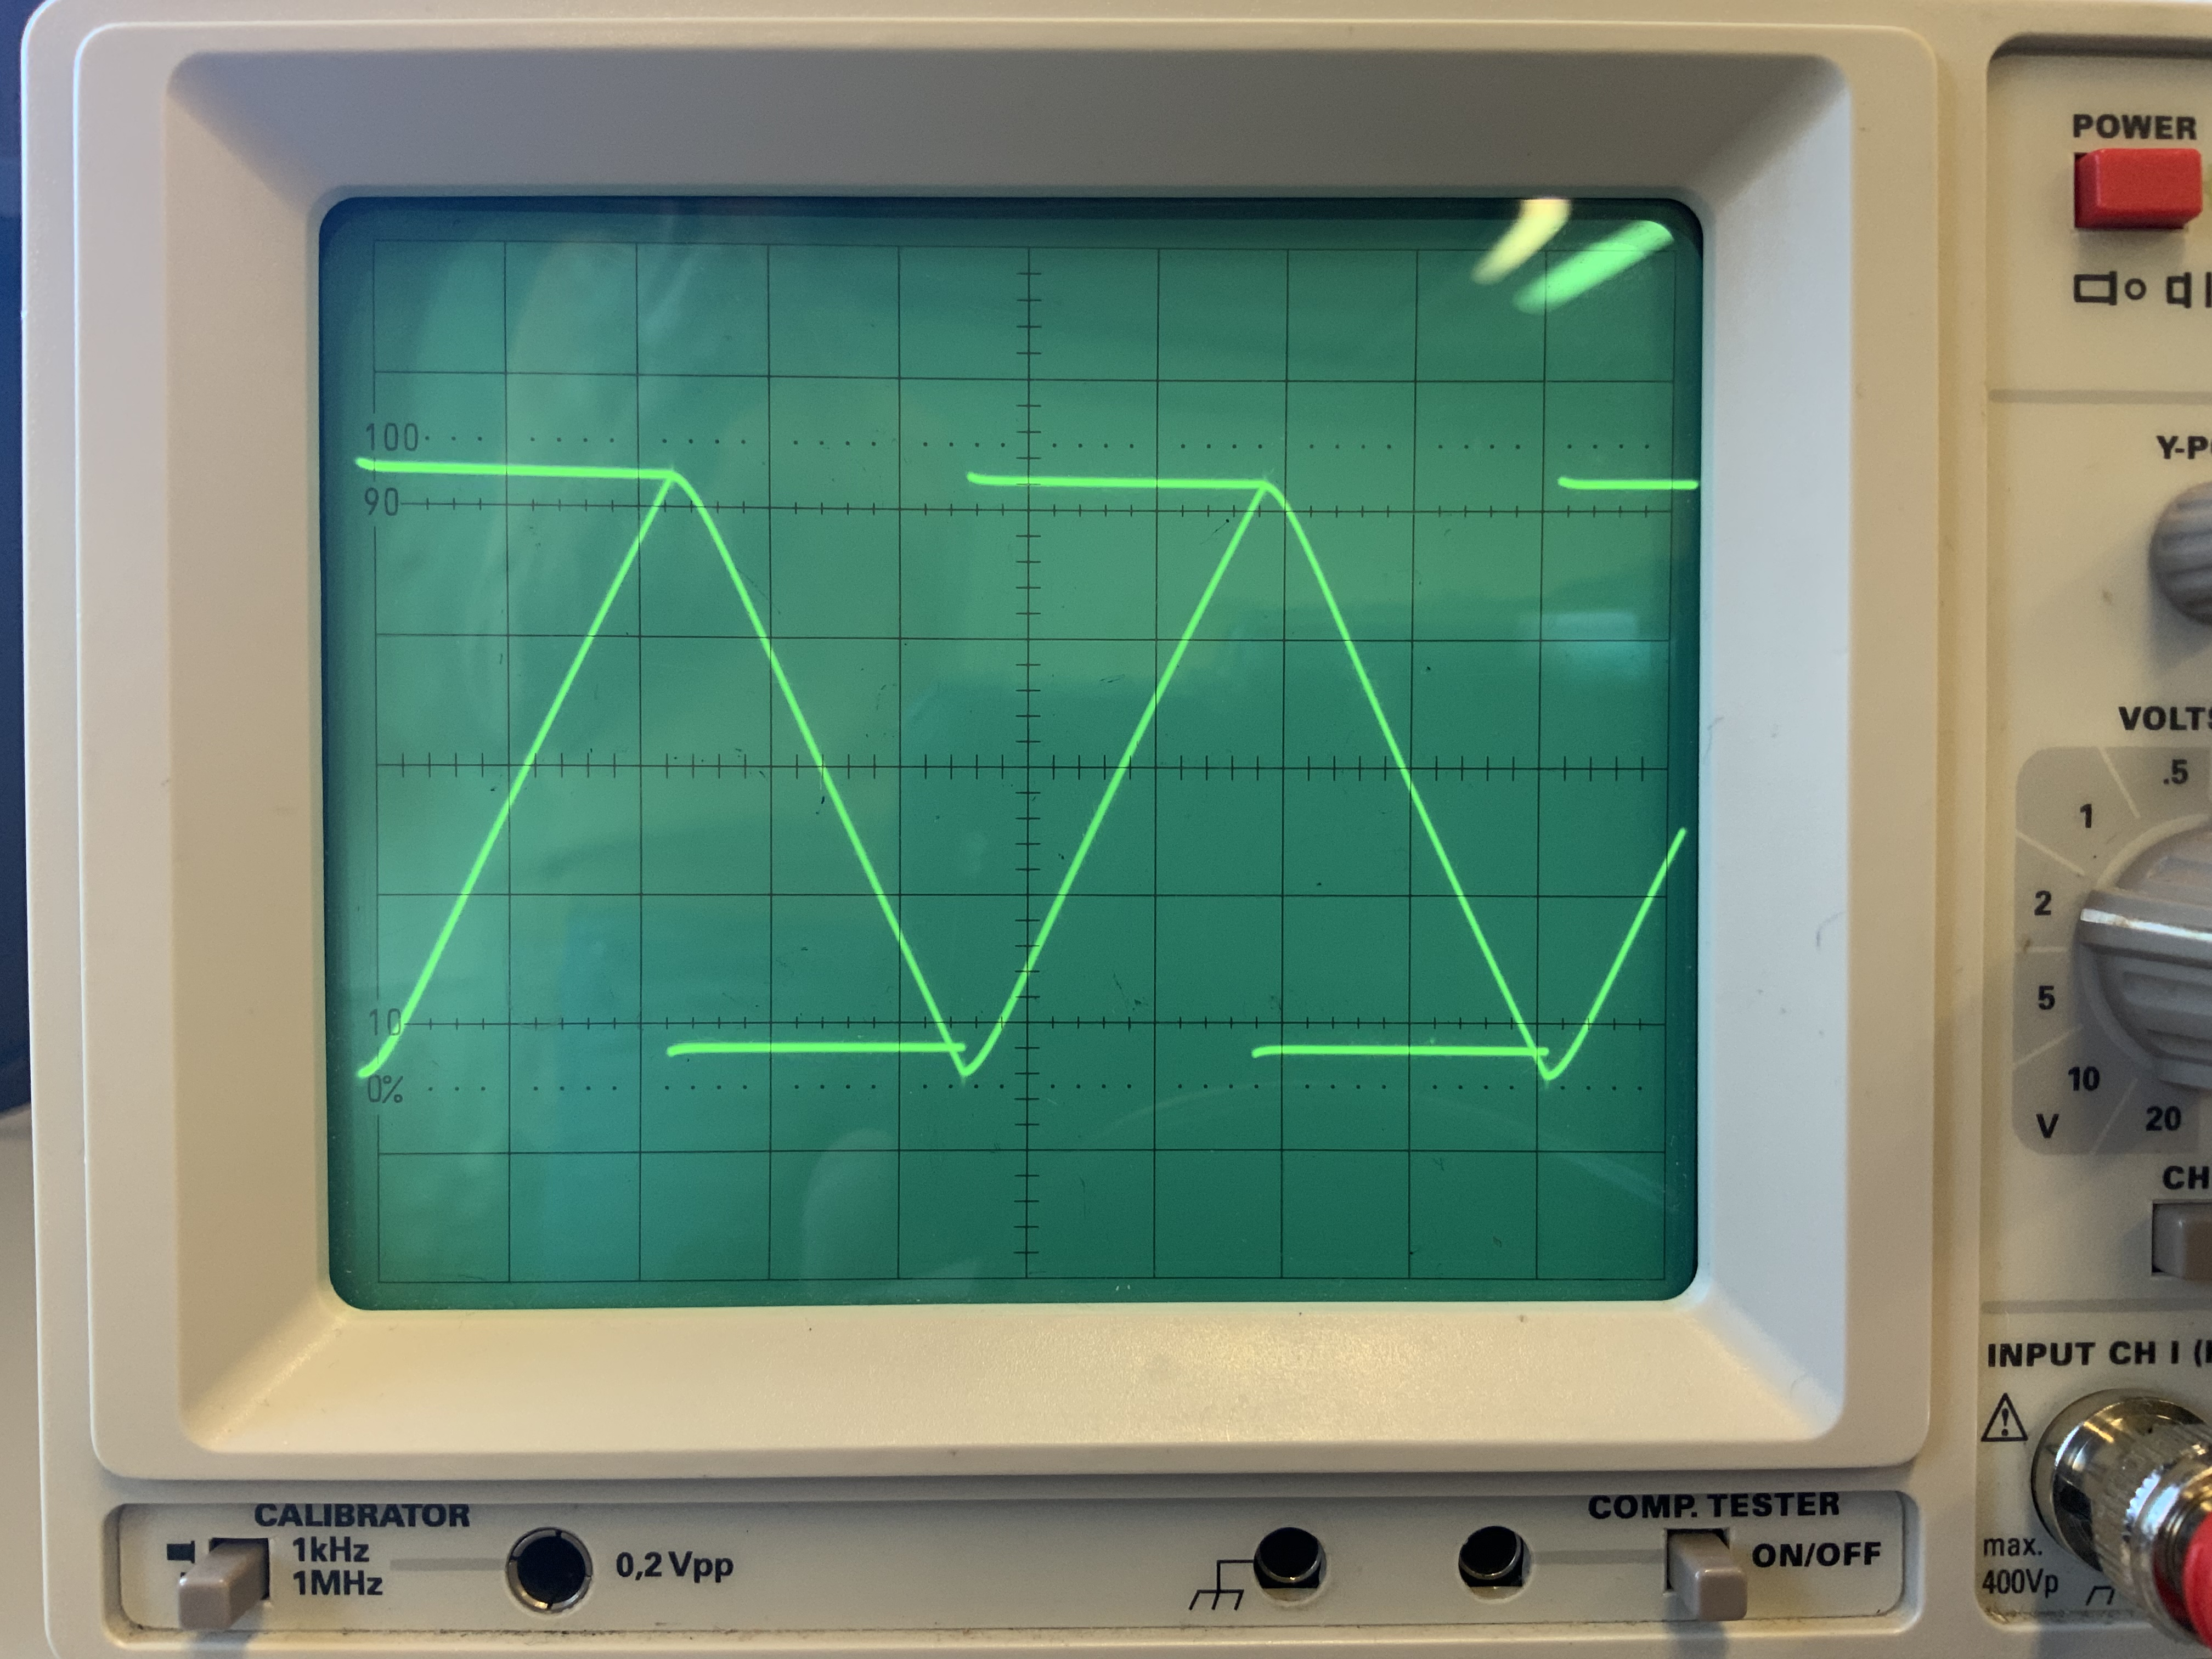
\includegraphics[width=0.75\textwidth]{Dateien/d.3.jpeg}
    \caption{Angelegte Rechteckspannung am RC-Kreis.}
    \label{fig:d.3}
\end{figure}
\begin{figure}[H]
    \centering
    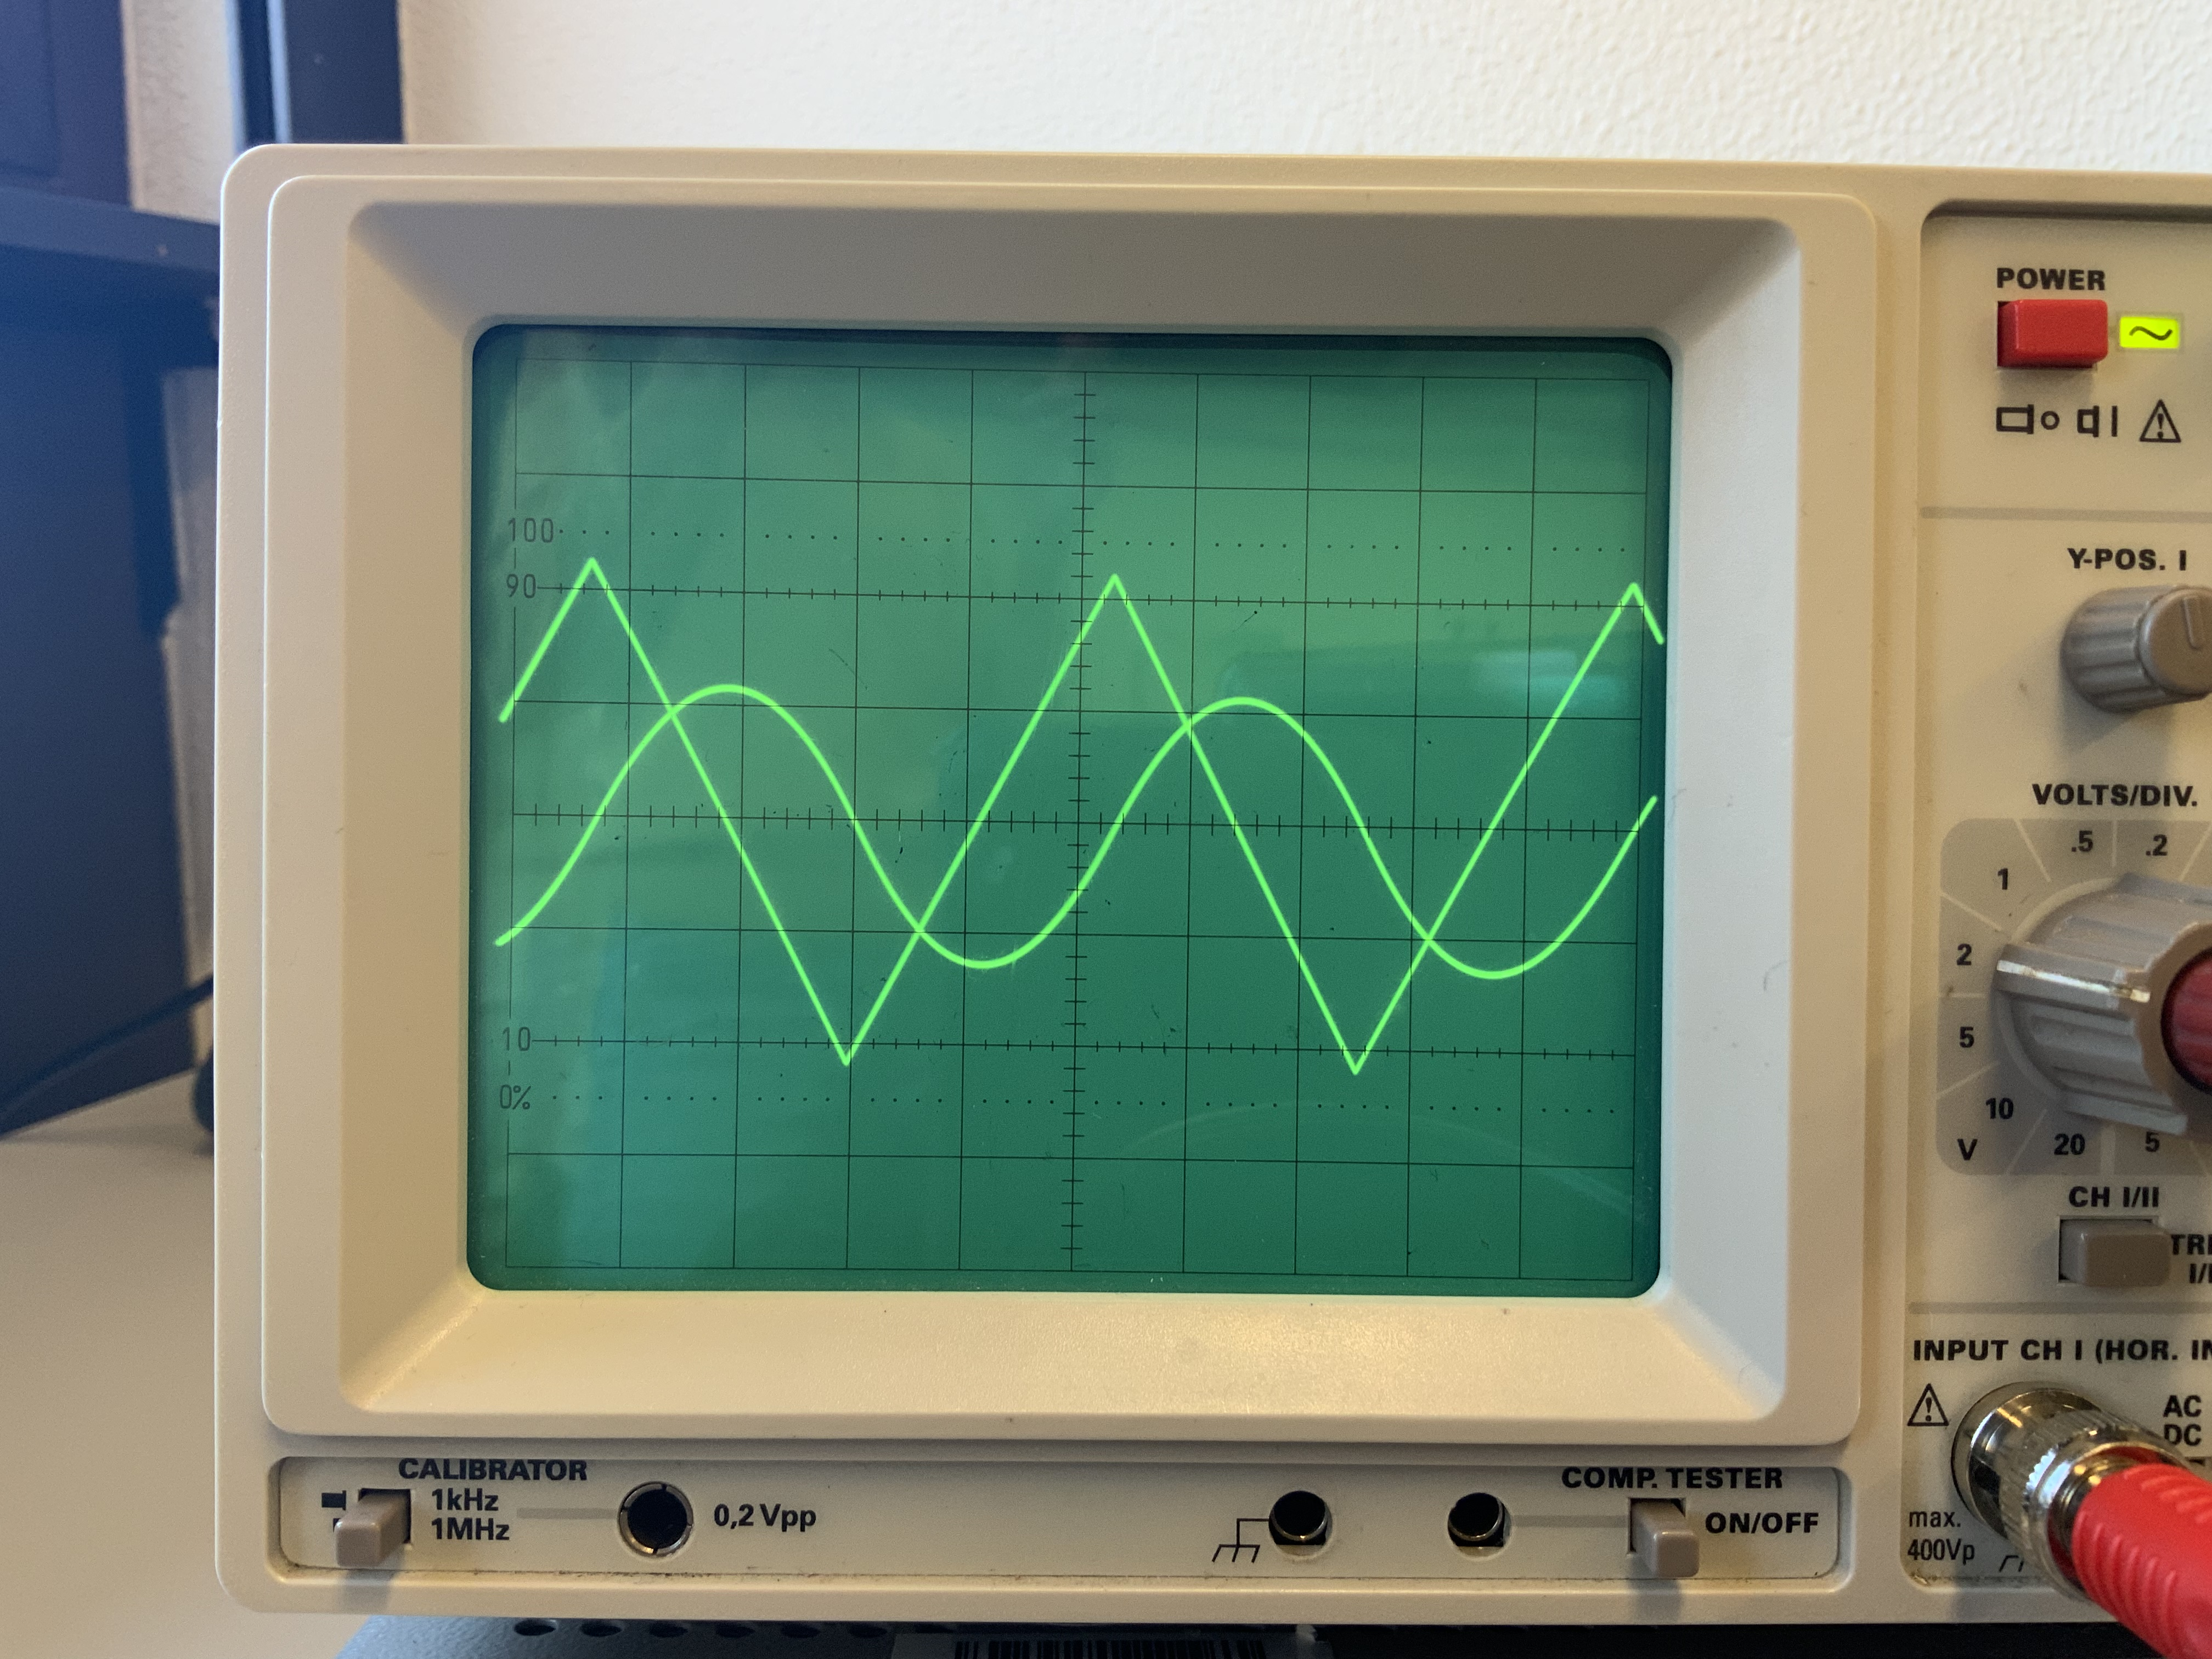
\includegraphics[width=0.75\textwidth]{Dateien/d.2.jpeg}
    \caption{Angelegte Dreiecksspannung am RC-Kreis.}
    \label{fig:d.2}
\end{figure}
\begin{figure}[H]
    \centering
    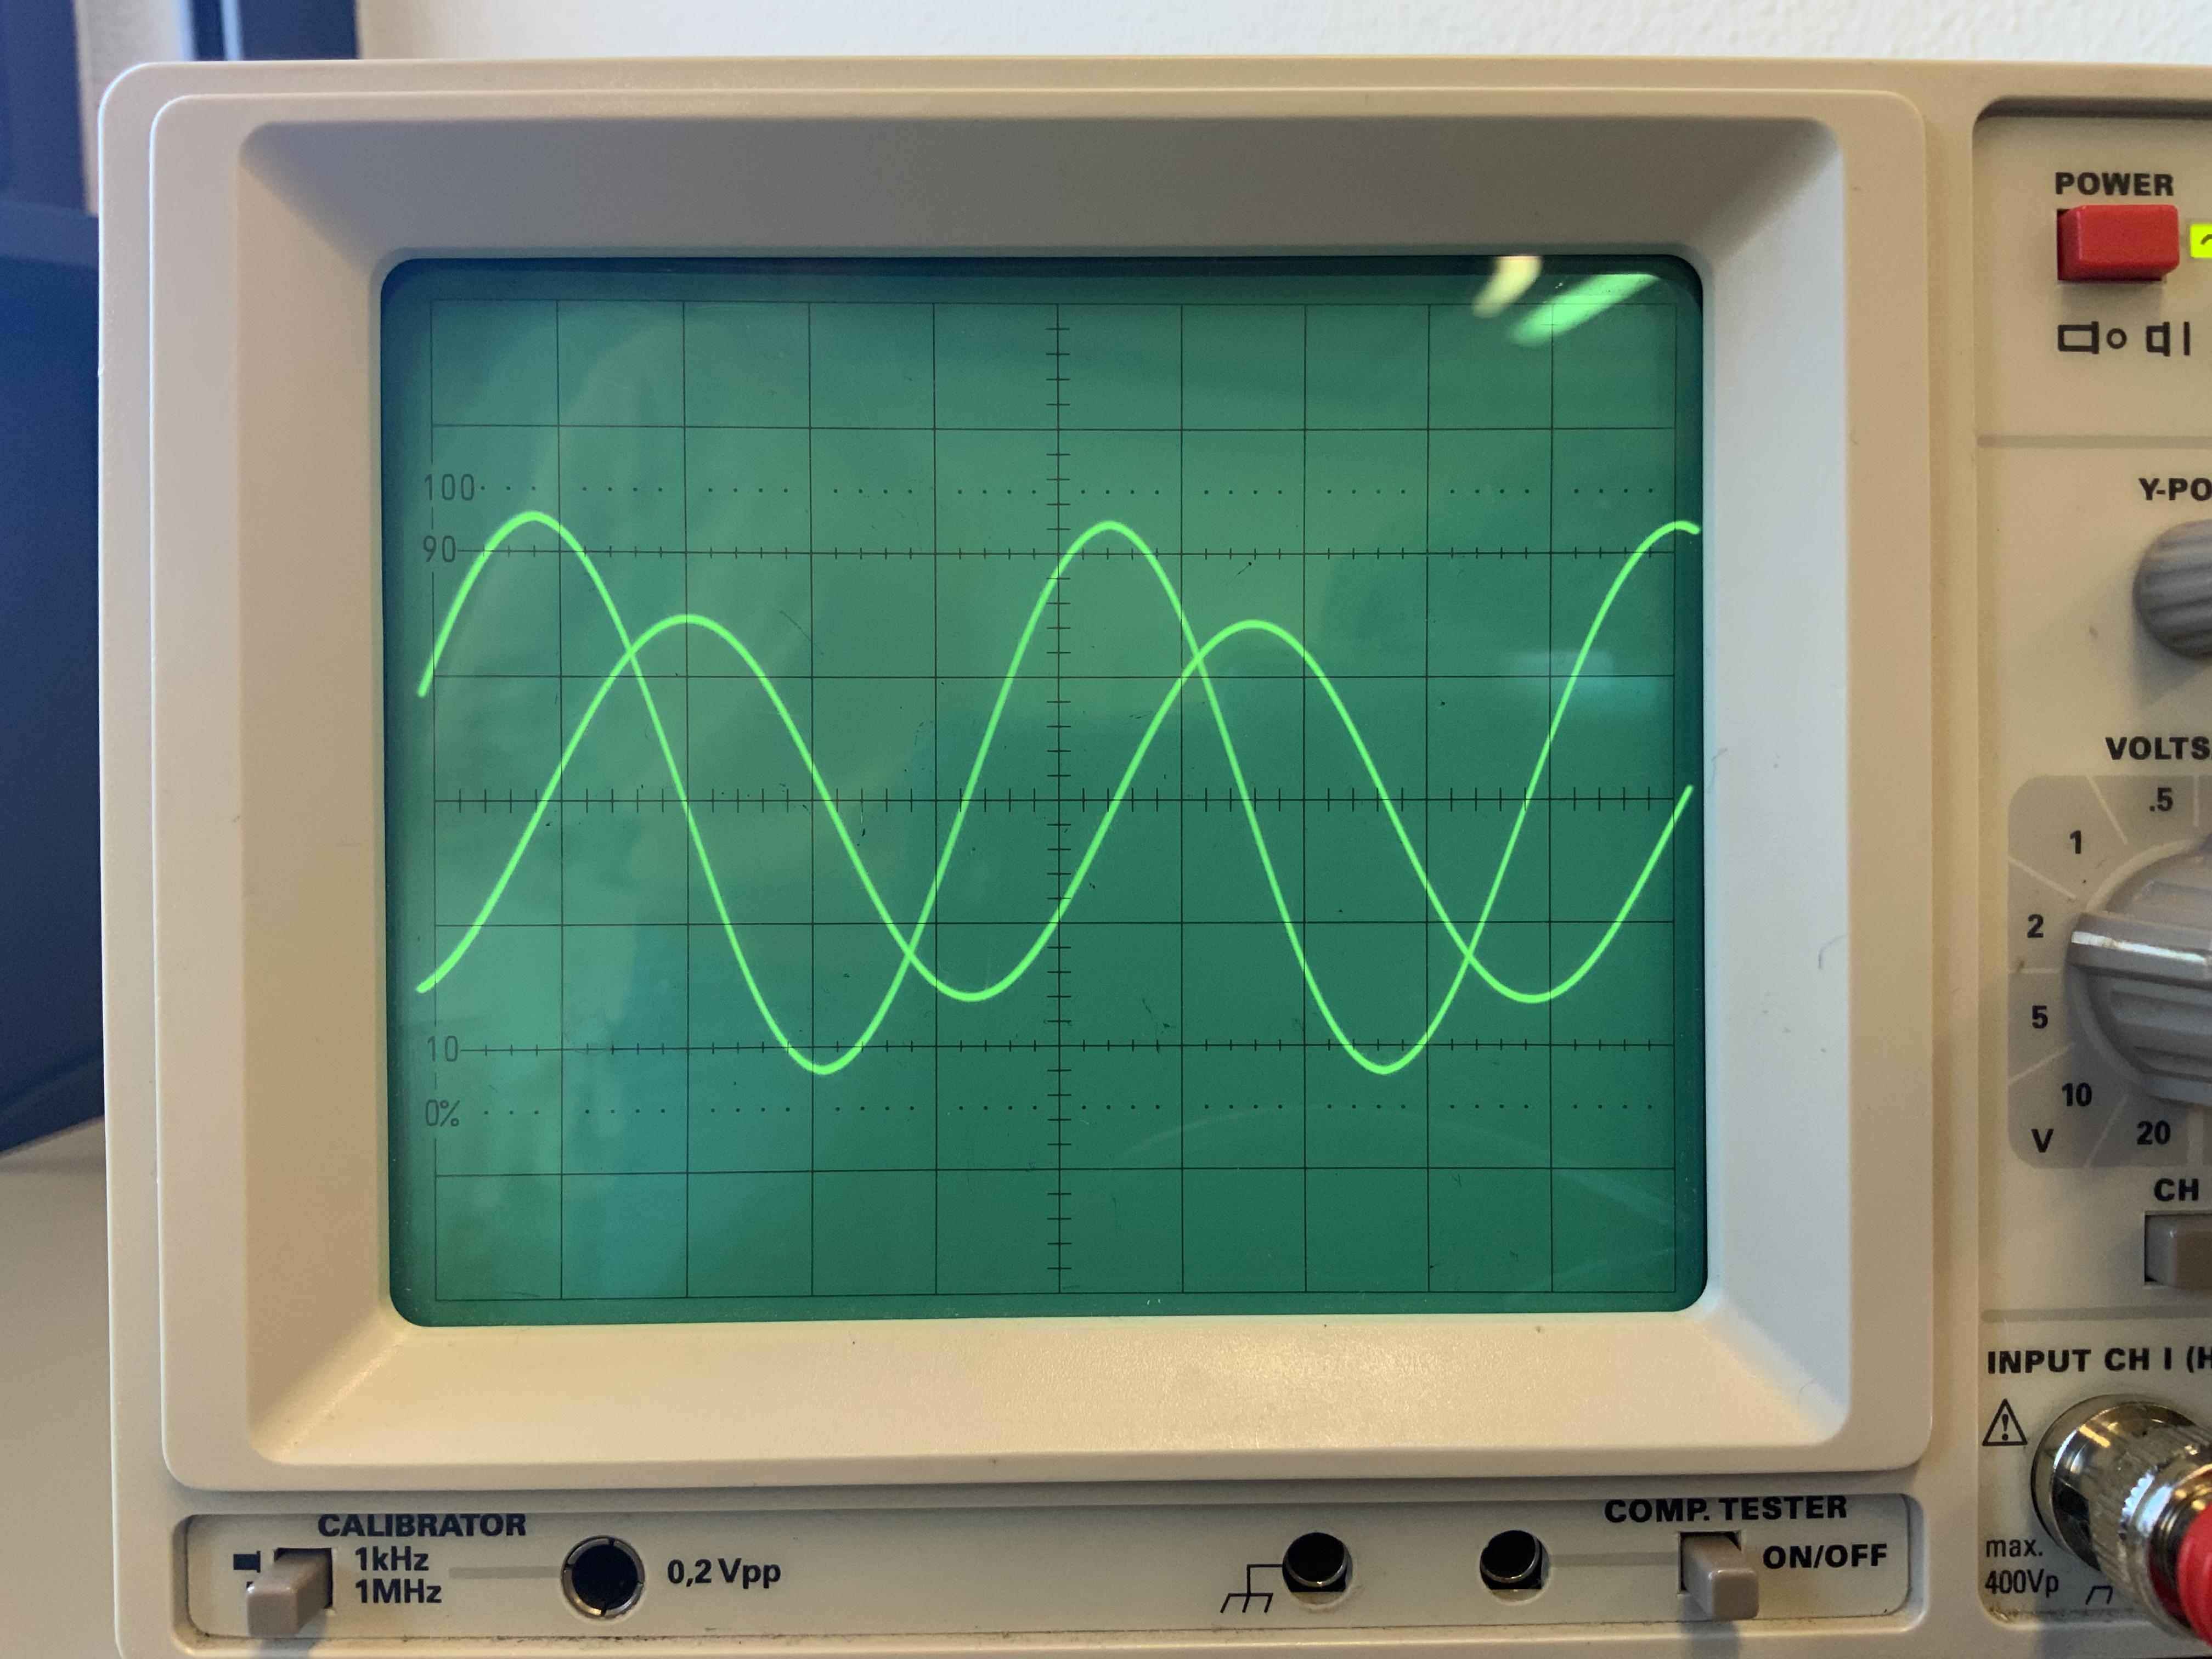
\includegraphics[width=0.75\textwidth]{Dateien/d.1.jpeg}
    \caption{Angelegte Sinusspannung am RC-Kreis.}
    \label{fig:d.1}
\end{figure}
\newpage
\section{Diskussion}
\label{sec:Diskussion}


Die Messwerte unterscheiden sich zum Teil recht stark von den Theoriewerten, was vermutlich daran liegt, dass große Messfehler
in die Berechnung der Werte eingegangen ist. So wurde beim Messen der Durchmesser der jeweiligen Körperteile nicht auf die unterschiedlich
breiten Einzelteile eingegangen (beim Arm zum Beispiel bei Ober- und Unterarm), sondern ein Mittelwert für den Durchmesser des gesamten
Körperteiles genommen.

Ein weiterer großer Faktor für Abweichungen von den Theoriewerten ist das Messen der Periodendauer. Zum Stoppen der Zeit einer 
Periodendauer wurde eine Stoppuhr verwendet, die manuell ausgelöst und gestoppt werden musste. Durch menschliche Verfehlungen, wie zum Beispiel
der Reaktionszeit, wurden die Zeiten verfälscht. Es wurde zwar versucht durch eine höhere Anzahl an Messungen dieser Unsicherheit vorzubeugen, jedoch
spielt sie dennoch in das Endergebnis mit ein. 

%Die Abweichung bei der Bestimmung des Trägheitsmomentes der Kugel beträgt $17.6953 \%$ und die bei dem Zylinder $16.2894 \%$. Es lässt sich,
%unter Berücksichtigung der eingegangenen Fehler sagen, dass der Wert der Abweichung dennoch recht groß ist. Eigentlich war zu erwarten, dass sich die
%prozentuale Abweichung auf unter $10 \%$ beläuft. Entweder sind, entgegen den Erwartungen, schlechte Messwerte vorgenommen worden, oder es handelt
%sich um einen systematischen Fehler zum Beispiel von der Messapparatur.

%Die Abweichungen bei der Bestimmung der Trägheitsmomente der Puppe in verschiedenen Stellungen ist mit $41.33 \%$ bei der ersten Stellung und mit
%$37.49 \%$ allerdings noch höher. 

Es müssen die Näherungen der Puppe miteinbezogen werden. So wurden alle
Körperteile, auch der Kopf, auf Zylinder approximiert. Auch wurde für die Gliedmaßen nicht beide einzelne Glieder gemessen und dessen Trägheitsmomente
berechnet, sondern wurde für ein Glied das Trägheitsmoment exemplarisch bestimmt und in dem Gesamtträgheitsmoment doppelt einbezogen.

Bei den Apparatekonstanten wurde das Trägheitsmoment auf \newline
$I_{\text{D}} = (2,999 \pm 0,183) \cdot 10^{-3} \si{\kilogram\meter^2}$ und die
Winkelrichtgröße auf $(0,01821\pm 0,00082) \si{\newton\meter}$ bestimmt.
Die theoretischen Trägheitsmomente der Kugel und des Zylinders sind
\begin{align*}
    I_{\text{Zylinder,Theorie}} &= 0.349 \cdot 10^{-3} \si{\kilogram\meter^2}, \\
    I_{\text{Kugel,Theorie}} &= 1.306 \cdot 10^{-3} \si{\kilogram\meter^2}. \\
\end{align*}
Und die Trägheitsmomente der beiden Körper, die aus den Schwingungsdauern berechnet wurden sind
\begin{align*}
    I_{\text{Zylinder}} = (5,685 \pm 0,6501) \cdot 10^{-3} \si{\kilogram\meter^2}, \\
    I_{\text{Kugel}} = (23,110 \pm 2,4260) \cdot 10^{-3} \si{\kilogram\meter^2}. \\
\end{align*}
Dies entspricht einer Abweichung von $1628,94\%$ bei dem Zylinder und $1769.52\%$ bei der Kugel.

Die theoretischen Werte der einzelnen Körperteile und der Modellpuppe selbst, sind für die erste Stellung
\begin{align*}
    I_{\text{Arm}} &= 0.70351 \si{\kilogram\meter^2}, \\
    I_{\text{Kopf}} &= 0.715769 \si{\kilogram\meter^2}, \\
    I_{\text{Bein}} &= 0.127145 \si{\kilogram\meter^2}, \\
    I_{\text{Torso}} &= 0.229718 \si{\kilogram\meter^2}, \\
    I_{\text{Puppe,1}} &= 2.60682 \si{\kilogram\meter^2}. \\
\end{align*}
Für die zweite Stellung sind die Werte
\begin{align*}
    I_{\text{Arm}} &= 0.70351 \si{\kilogram\meter^2}, \\
    I_{\text{Kopf}} &= 0.715769 \si{\kilogram\meter^2}, \\
    I_{\text{Bein}} &= 1.20679 \si{\kilogram\meter^2}, \\ 
    I_{\text{Torso}} &= 0.229718 \si{\kilogram\meter^2}, \\
    I_{\text{Puppe,2}} &= 4.76611 \si{\kilogram\meter^2}.
\end{align*}
Und die Trägheitsmomente aus den Schwingungsdauern sind
\begin{align*}
    I_{1} &= (0,3055\pm 0,03100) \cdot 10^{-3} \si{\kilogram\meter^2}, \\
    I_{2} &= (0,5669\pm 0,05034) \cdot 10^{-3} \si{\kilogram\meter^2}.
\end{align*}
Das entspricht einer Abwertung des experimentellen Wertes von dem Theoriewert um $41.33 \%$ für die erste Stellung und
$37.49 \%$ für die zweite Stellung.

Es ergibt sich ein Verhältnis für den theoretischen Wert der beiden Stellungen zu
\begin{align}
    \frac{I_1}{I_2} = &= 0,5469\pm 0,07.
\end{align}
Und für den experimentellen Wert
\begin{align*}
    \frac{I_1}{I_2} = &= 0,5389\pm 0,07.
\end{align*}
Dies entspricht einer Genauigkeit von $1,46\%$.

Da bei der Puppe so viele Approximierungen vorgenommen wurden ist allerdings daon auszugehen, dass der experimentell bestimmte Wert näher am 
tatsächlichen Wert ist, als der theoretisch bestimmte Wert.
\section{Anhang}
\label{sec:anhang}

\begin{figure}
    \centering
    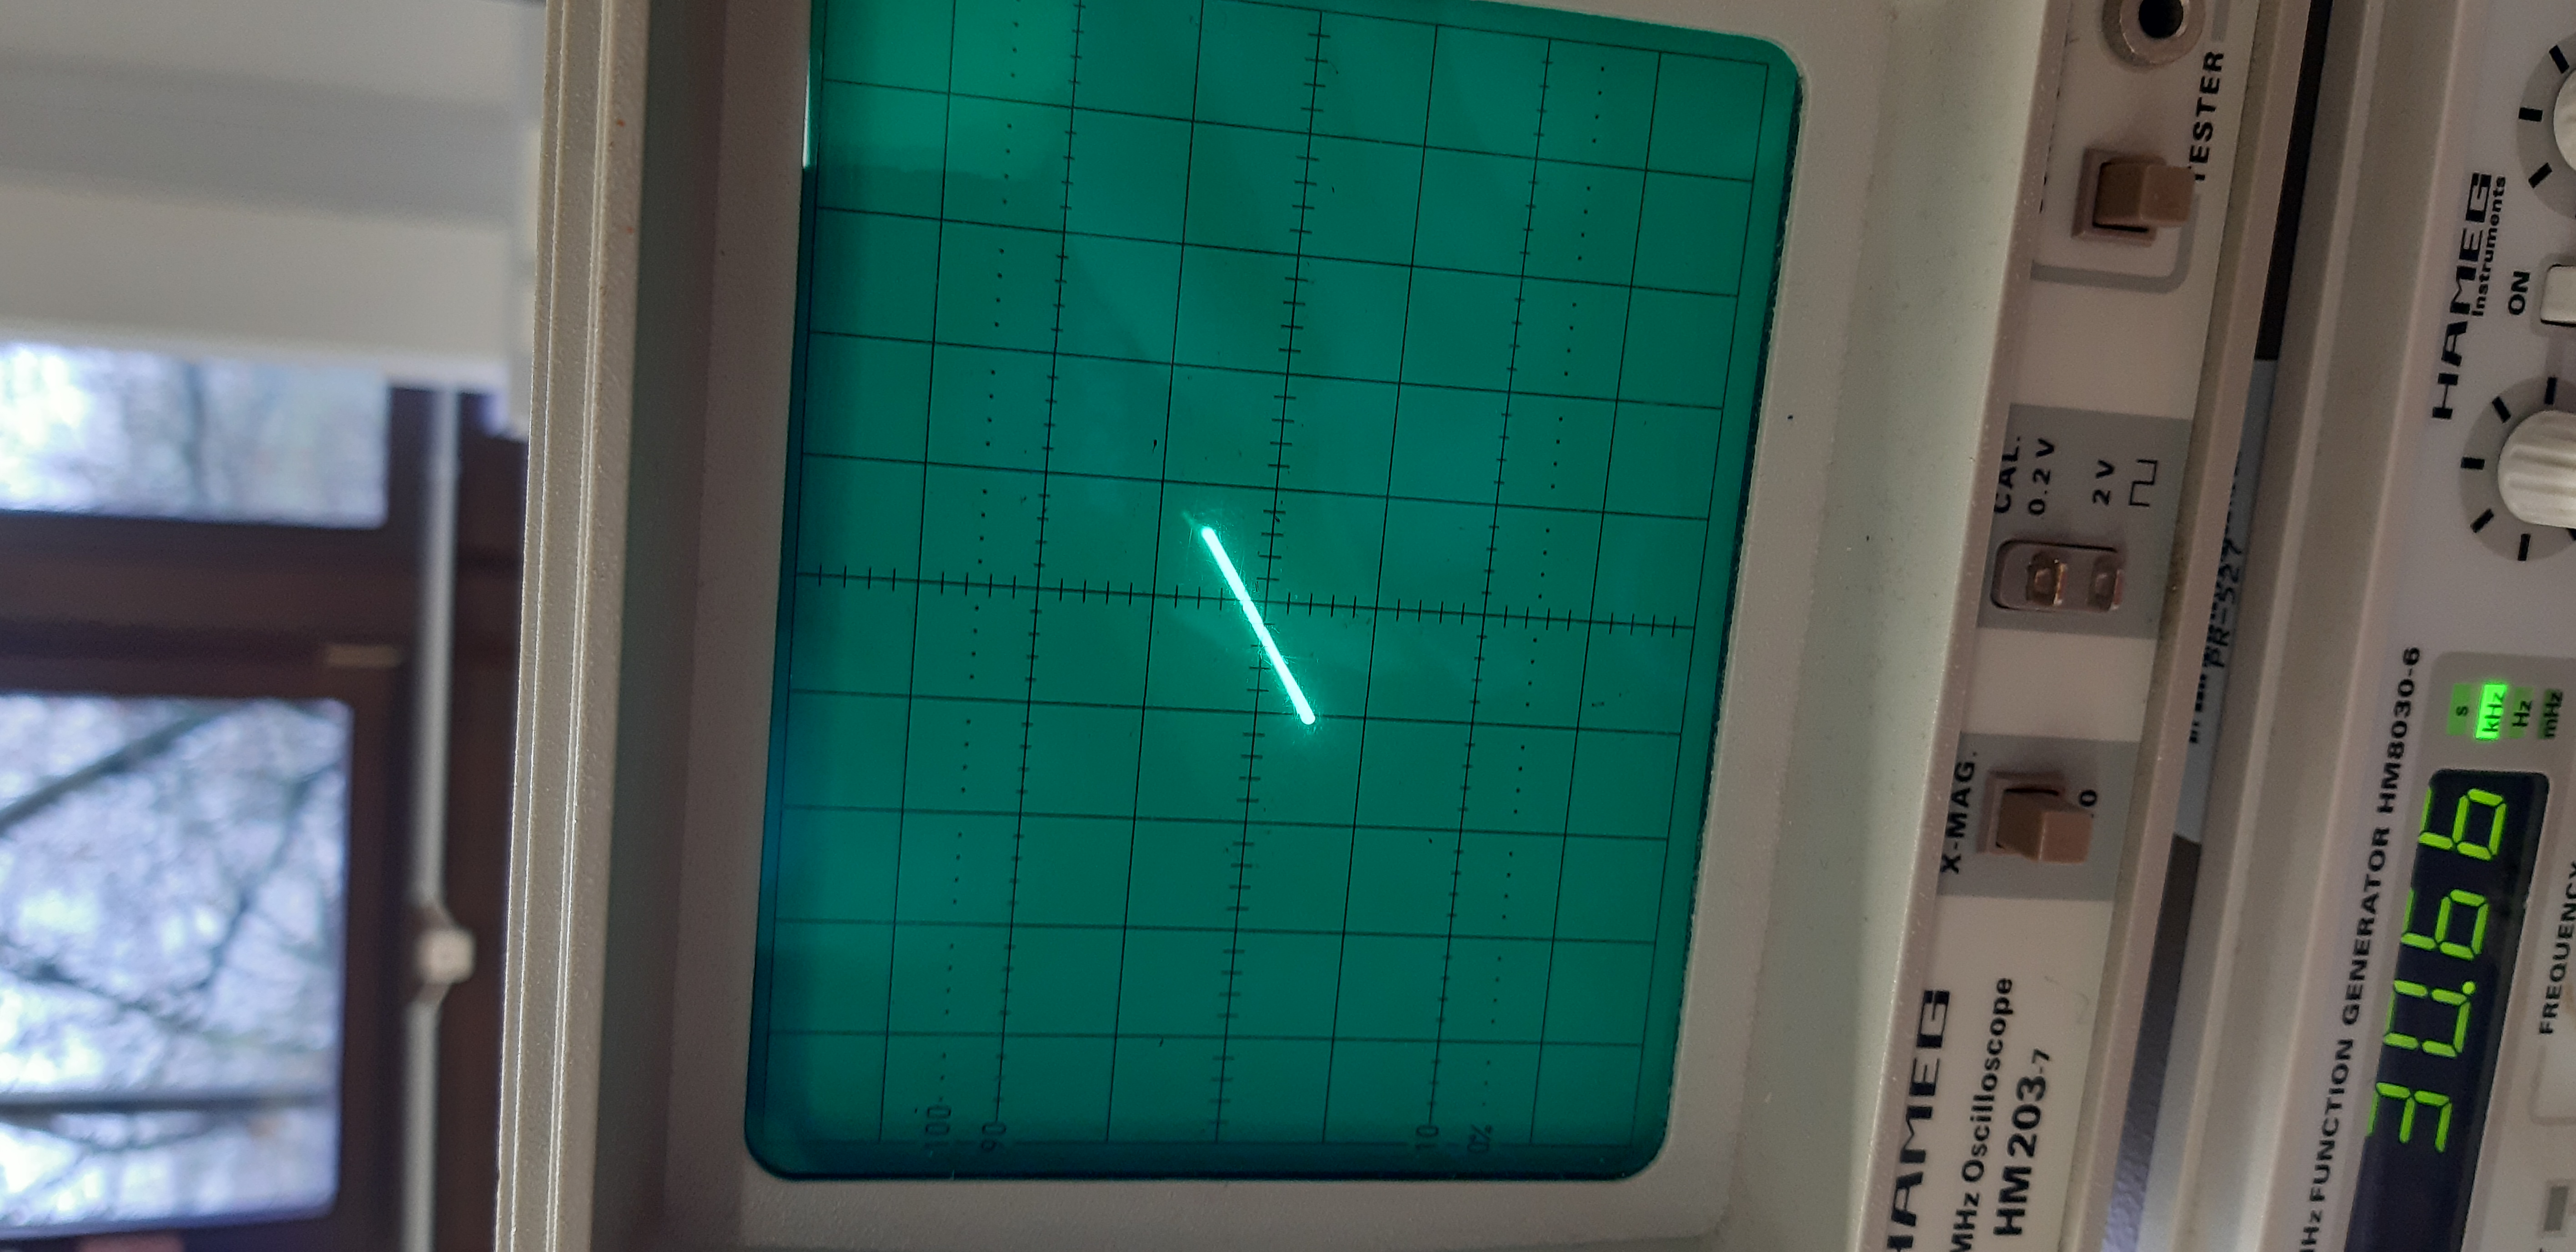
\includegraphics[width=0.75\textwidth, angle=-90]{plots/Lissajour-Gerade.jpeg}
    \caption{Lissajous-Figur der Justierung.}
    \label{fig:Lissajous}
\end{figure}

\begin{figure}
    \centering
    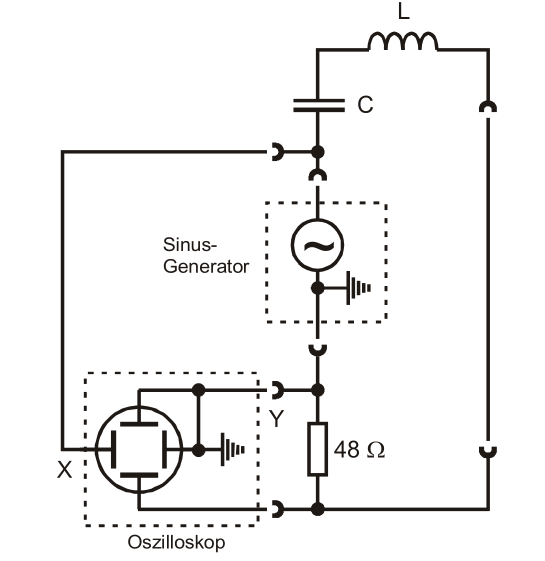
\includegraphics[width=0.75\textwidth]{plots/Schaltung0.png}
    \caption{Schaltung zur Einstellung der Resonanzfrequenz \cite{Versuchsanleitung}}
    \label{fig:schaltung0}
\end{figure}

\begin{figure}
    \centering
    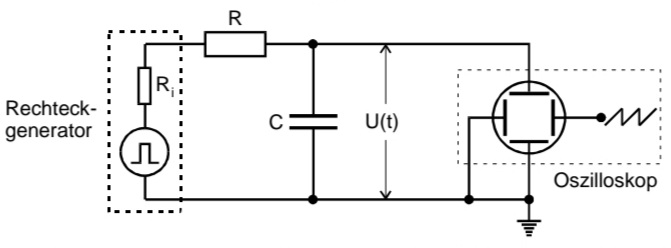
\includegraphics[width=0.75\textwidth]{plots/Schaltung1.png}
    \caption{Schaltung für den Austausch der Schwingungsenergie \cite{Versuchsanleitung}}
    \label{fig:schaltung1}
\end{figure}

\printbibliography{}

\end{document}
